\setchapterimage[7cm]{ic/ic_icecube.jpg}
\chapter{The IceCube Detector} \label{ic}
\labch{IceCube}
One of the two most relevant instruments for this thesis is the \textit{IceCube Detector}, a neutrino detector located at the geographic South Pole. It is the successor to the Antarctic Muon And Neutrino Detector Array (AMANDA) at the same location \sidecite{Andres1999, Andres2000}. 
\begin{marginfigure}
    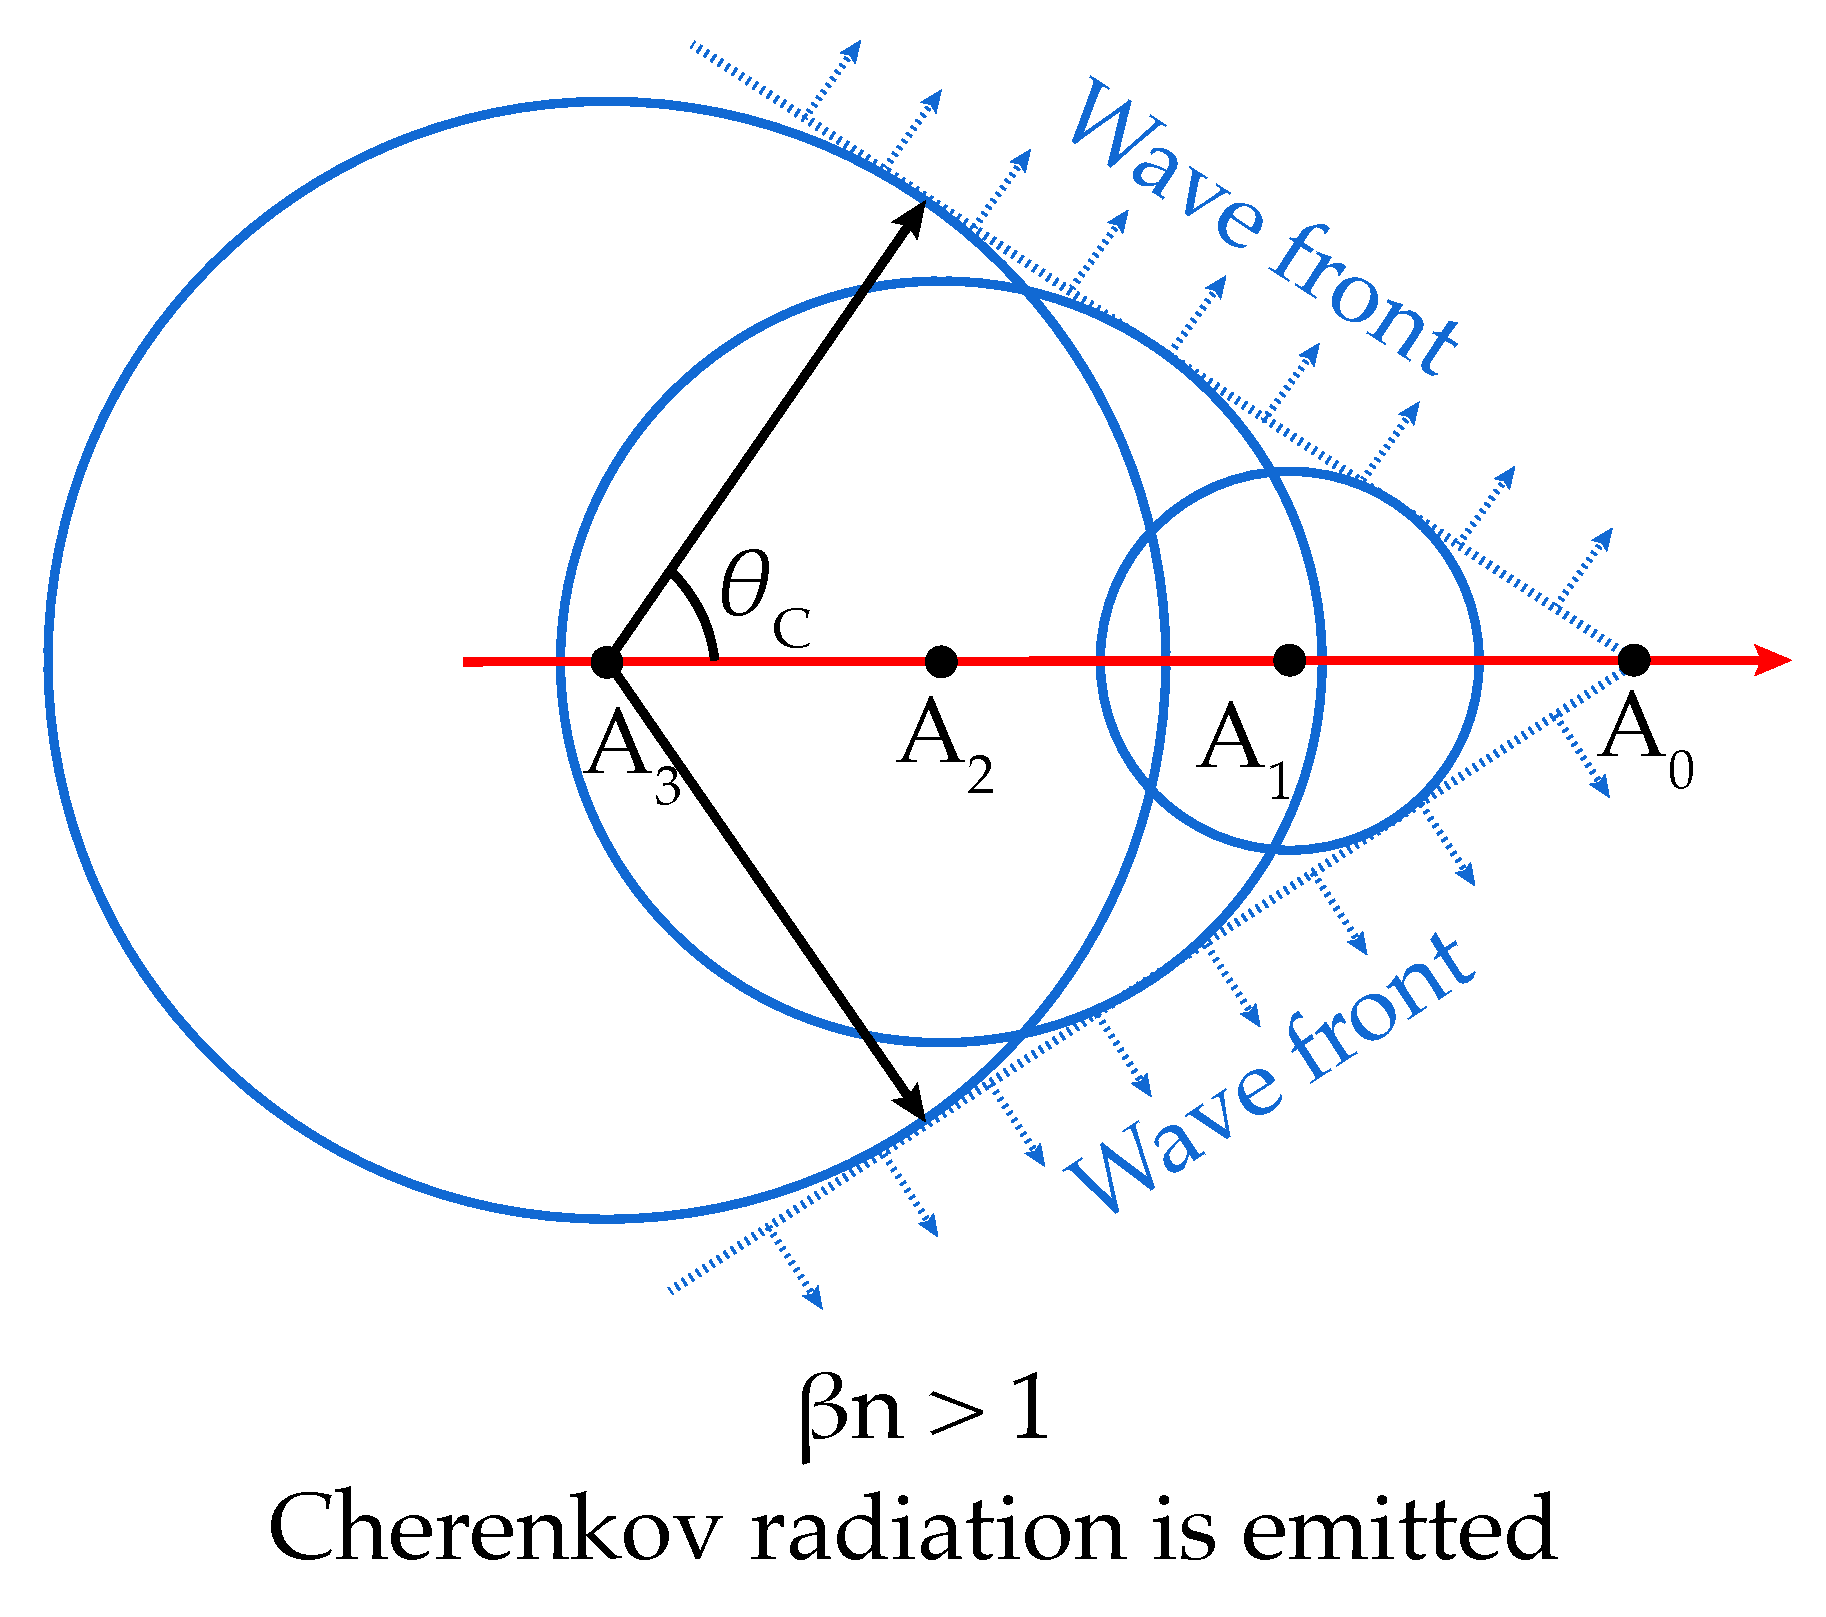
\includegraphics{ic/ic_cherenkov1.pdf}
    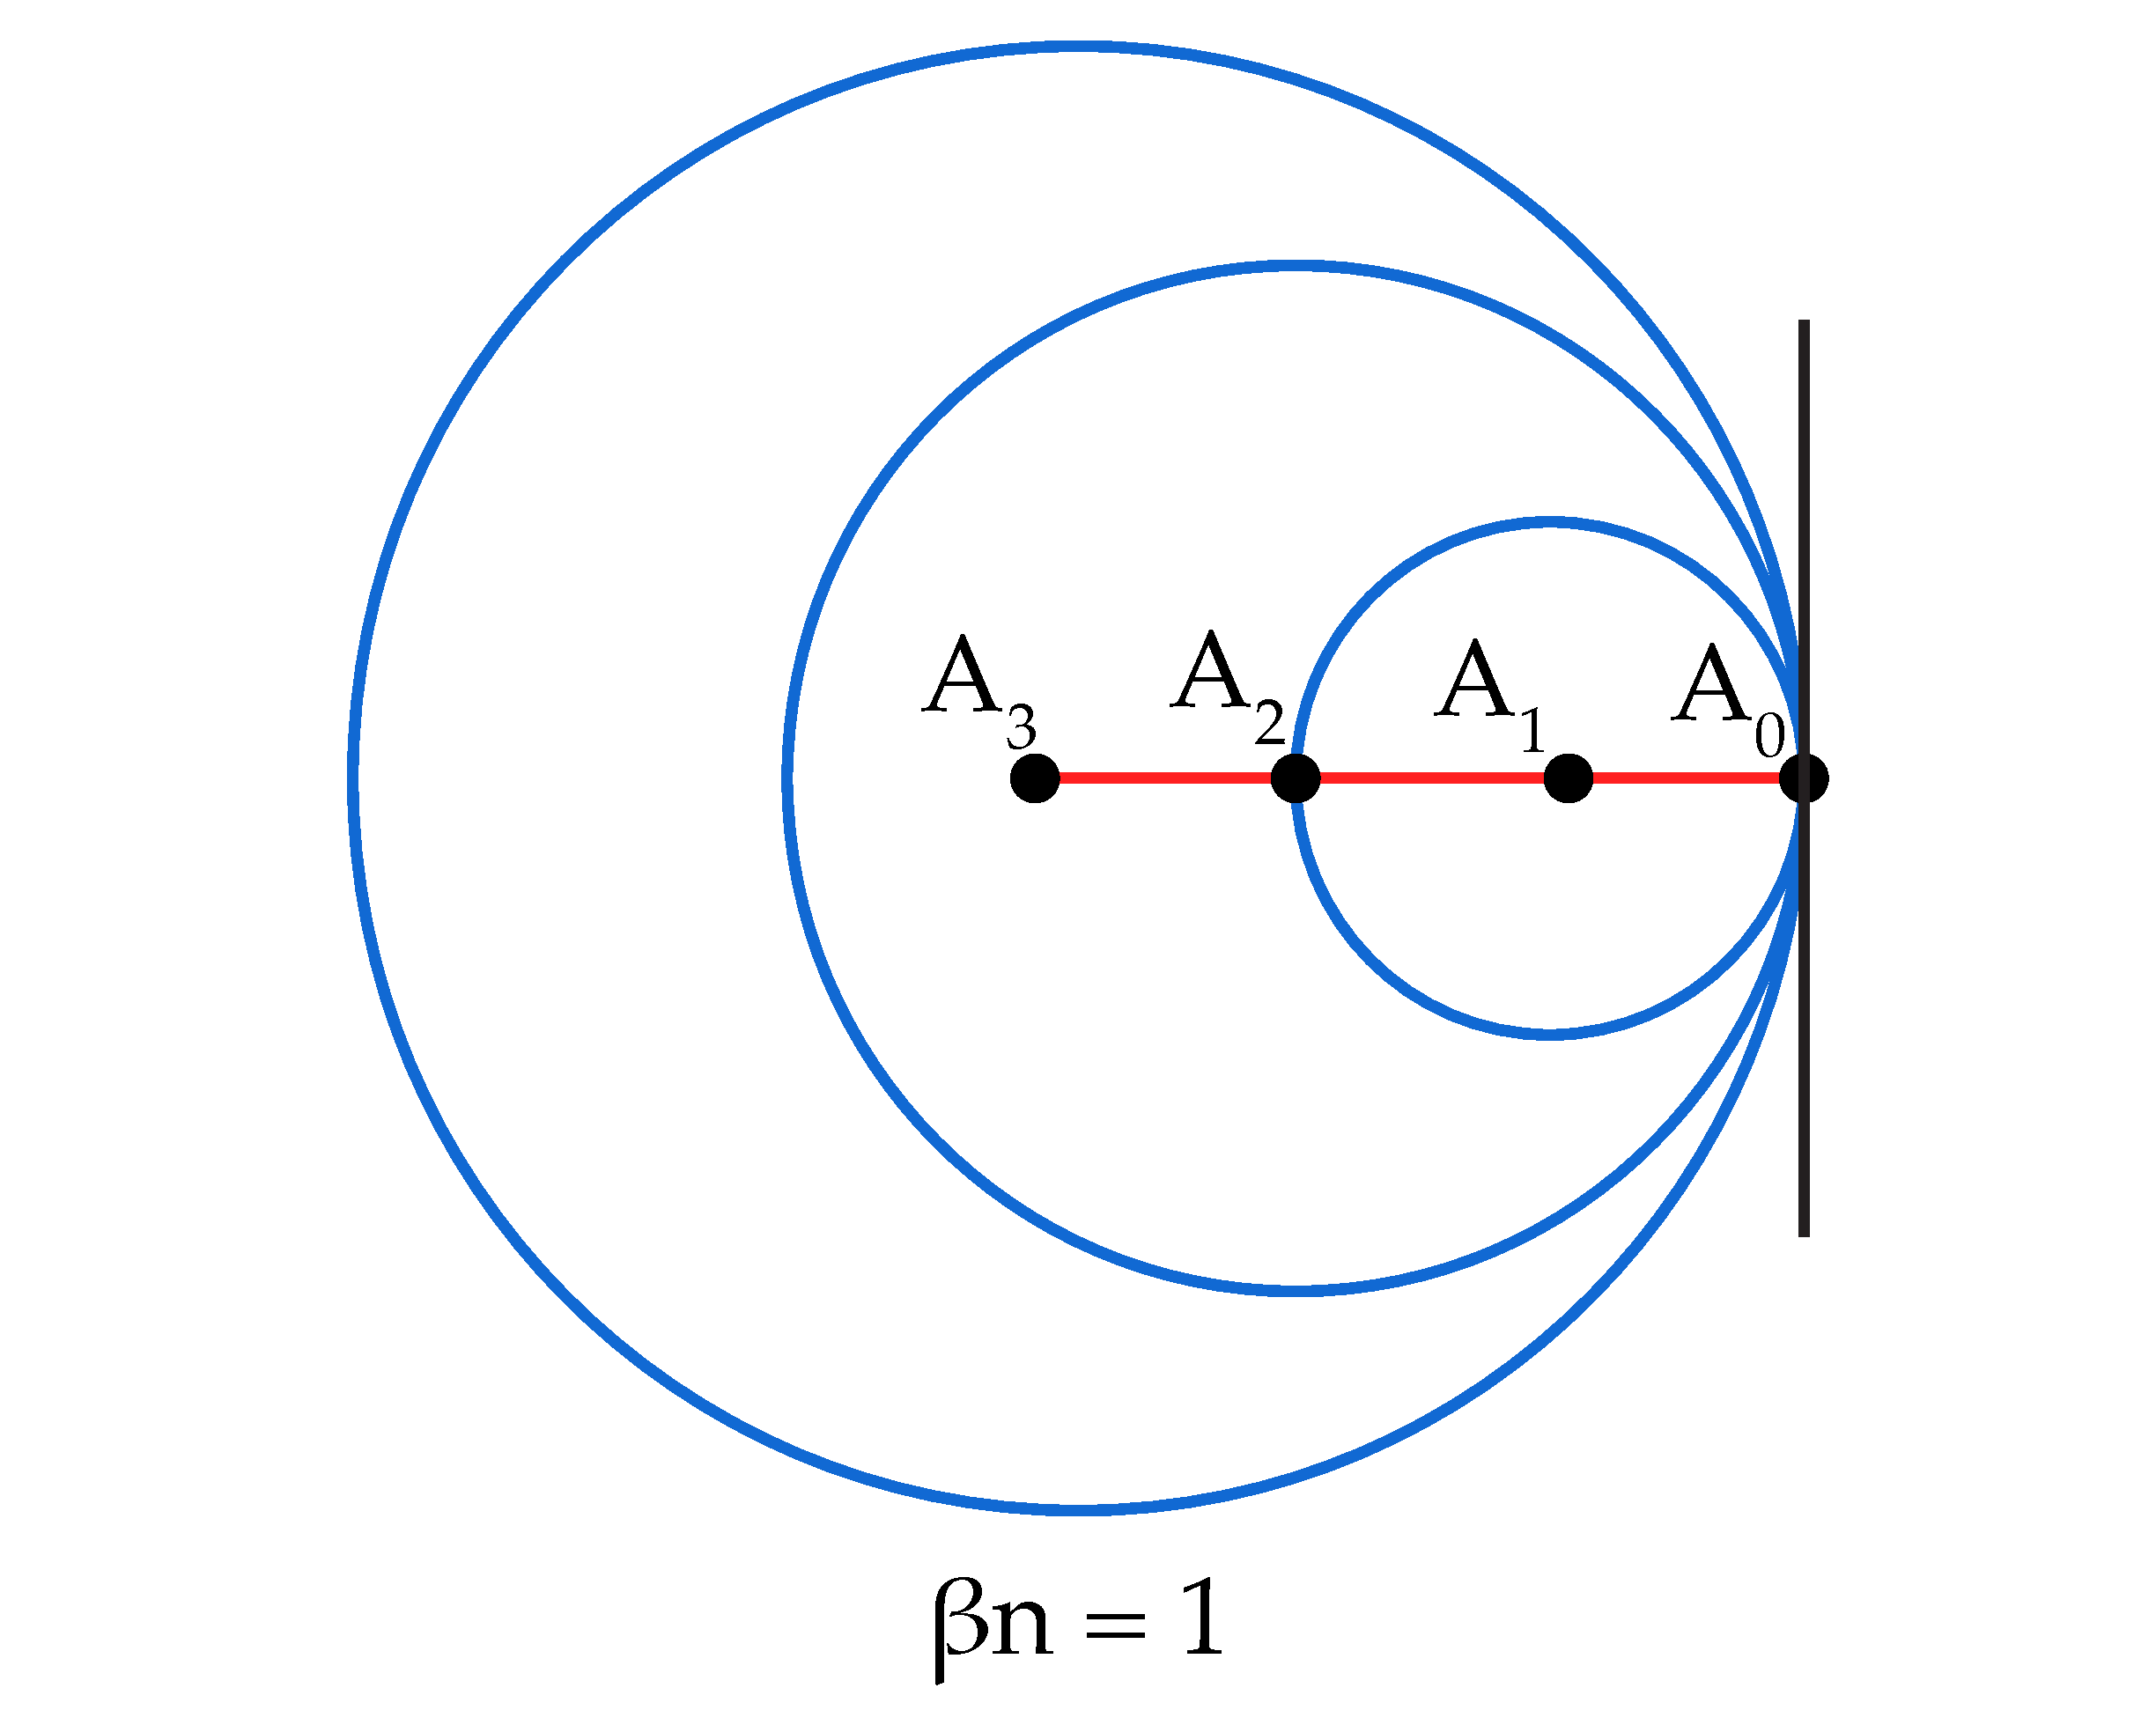
\includegraphics{ic/ic_cherenkov2.pdf}
    \caption[Cherenkov radiation]{The principle of Cherenkov radiation. In the upper figure Cherenkov radiation is emitted at the Cherenkov angle $\theta_\text{C}$, as the radiation emitted at different points in time forms a mutual, cone-shaped wavefront. In the figure on the bottom, all radiation is cancelled out by destructive interference (all circles are subsets of the first on the left, as the particle is not moving faster than light in the medium). Adapted from \cite{LAnnunziata2020}.}
    \labfig{cherenkov}
\end{marginfigure}
The basic oeprational principle of IceCube (and already of AMANDA) is the detection of Cherenkov light within the Antarctic ice. When charged secondary particles created by neutrino interactions travel through the ice, their speed exceeds the phase velocity of light in ice and they emit Cherenkov radiation. The detector consists of 5160 individual digital optical modules (DOMs), buried deep in the ice and sensitive to the Cherenkov radiation.

\section{Cherenkov radiation} \label{cherenkov_radiation}

Cherenkov radation was first detected in 1934 by Soviet scientist Pavel Cherenkov \sidecite{Cherenkov1934}. It occurs when charged particles travel within a medium with a velocity exceeding the speed of light in that very medium. The refractive index in a medium is defined as $n=\frac{c_0}{c_m}$, where $c_m$ is the speed of light in vacuum and $c_m$ is the phase velocity of light in that medium. Note that the phase velocity of light in a medium can exceed $c_0$, so $n<1$ is possible. 

When charged particles cross an electrically neutral dielectric medium, atoms along the particle's path are briefly polarized. When they relax back to the ground state, the atoms emit electromagnetic radiation.

For slow particles, this radiation destructively interferes with itself, canceling out all signals (see the bottom panel of Fig. \ref{fig:cherenkov}). Now, if the particle is travelling faster than the speed of light within the medium $c_m$, this destructive interference does not happen. Rather, a cone-shaped wavefront gets created (see top panel of Fig. \ref{fig:cherenkov}). This wavefront constitutes Cherenkov radiation. If the particle has speed $v=\beta c_0$, the angle $\theta$ between the particle trajectory and the direction of the Cherenkov radiation can be calculated as \sidecite{LAnnunziata2020}:

\begin{equation}
\cos{\theta} = \frac{\beta}{n}
\end{equation}

For example: If the medium is ice, to first order the refractive index $n\approx1.31$.\sidenote{This is of course rather crude. The $n$ of Antarctic glacial ice depends e.g. on depth; a fact we will come back to later when discussing directional reconstruction of high-energy IceCube neutrinos.} A secondary muon traveling through the ice at $0.999\,c_0$ will therefore emit Cherenkov light at an angle of $\theta = \cos^{-1}{\big(\frac{0.999}{1.31}\big)} \approx \SI{40}{\degree}$. 
\begin{marginfigure}
    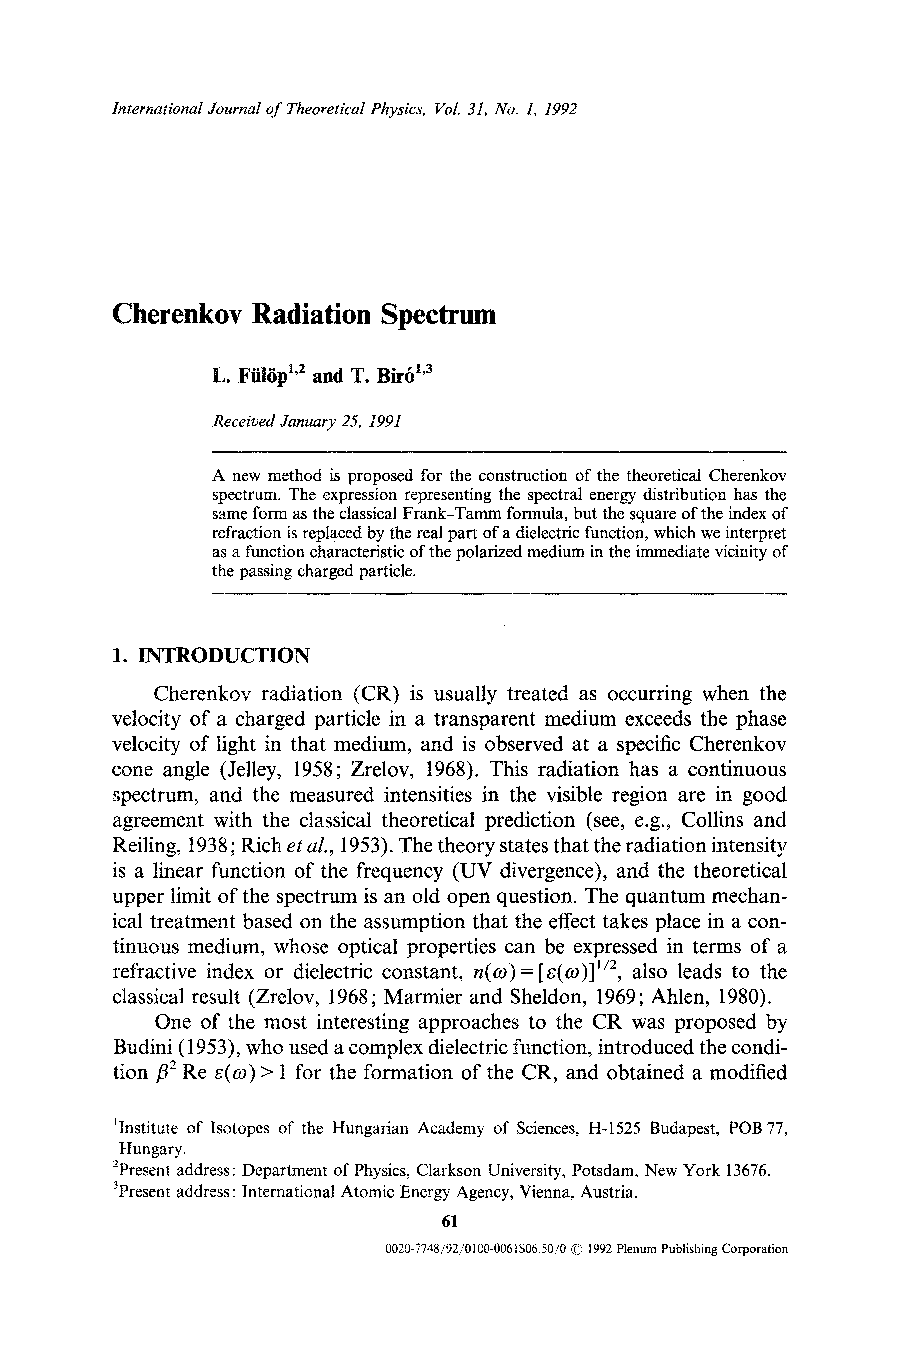
\includegraphics{ic/ic_cherenkov_spectrum.pdf}
    \caption[Cherenkov spectrum]{Cherenkov spectrum for a particle with $v=0.8 \,c_0$ in water. The intensity peaks at $\SI{4e15}{\Hz}$, corresponding to a wavelength of \SI{75}{\nm}, lying at the high-frequency end of the UV spectrum. Adapted from \cite{Fulop1992}.}
    \labfig{cherenkov_spectrum}
\end{marginfigure}
Cherenkov radiation does not have spectral peaks, but is continuous, with a relative intensity proportional to the frequency. Note that the refractive index of a medium also dpends on the frequency, dropping below 1 in the X-ray. From this it follows that Cherenkov radiation appears blue to the human eye (the high-frequency part dominates) and peaks in the ultra violet (UV), before it sharply drops off in the X-ray regime \sidecite{Fulop1992}, see Fig. \ref{fig:cherenkov_spectrum}.

\section{Instrumentation}

IceCube detects neutrinos by observing the optical part of their secondary particle Cherenkov spectrum (see Section \ref{cherenkov_radiation} above). To understand how this is done, one first needs to look at the working principe of a photomultiplier tube (PMT).

\subsection{Photomultiplier tubes}
A PMT is a device used to detect very faint light signals by amplifying them. They consist of vacuum tubes and were successfully realized for the first time in the 1930s \sidecite{Iams1935}.

\begin{figure}[h!]
    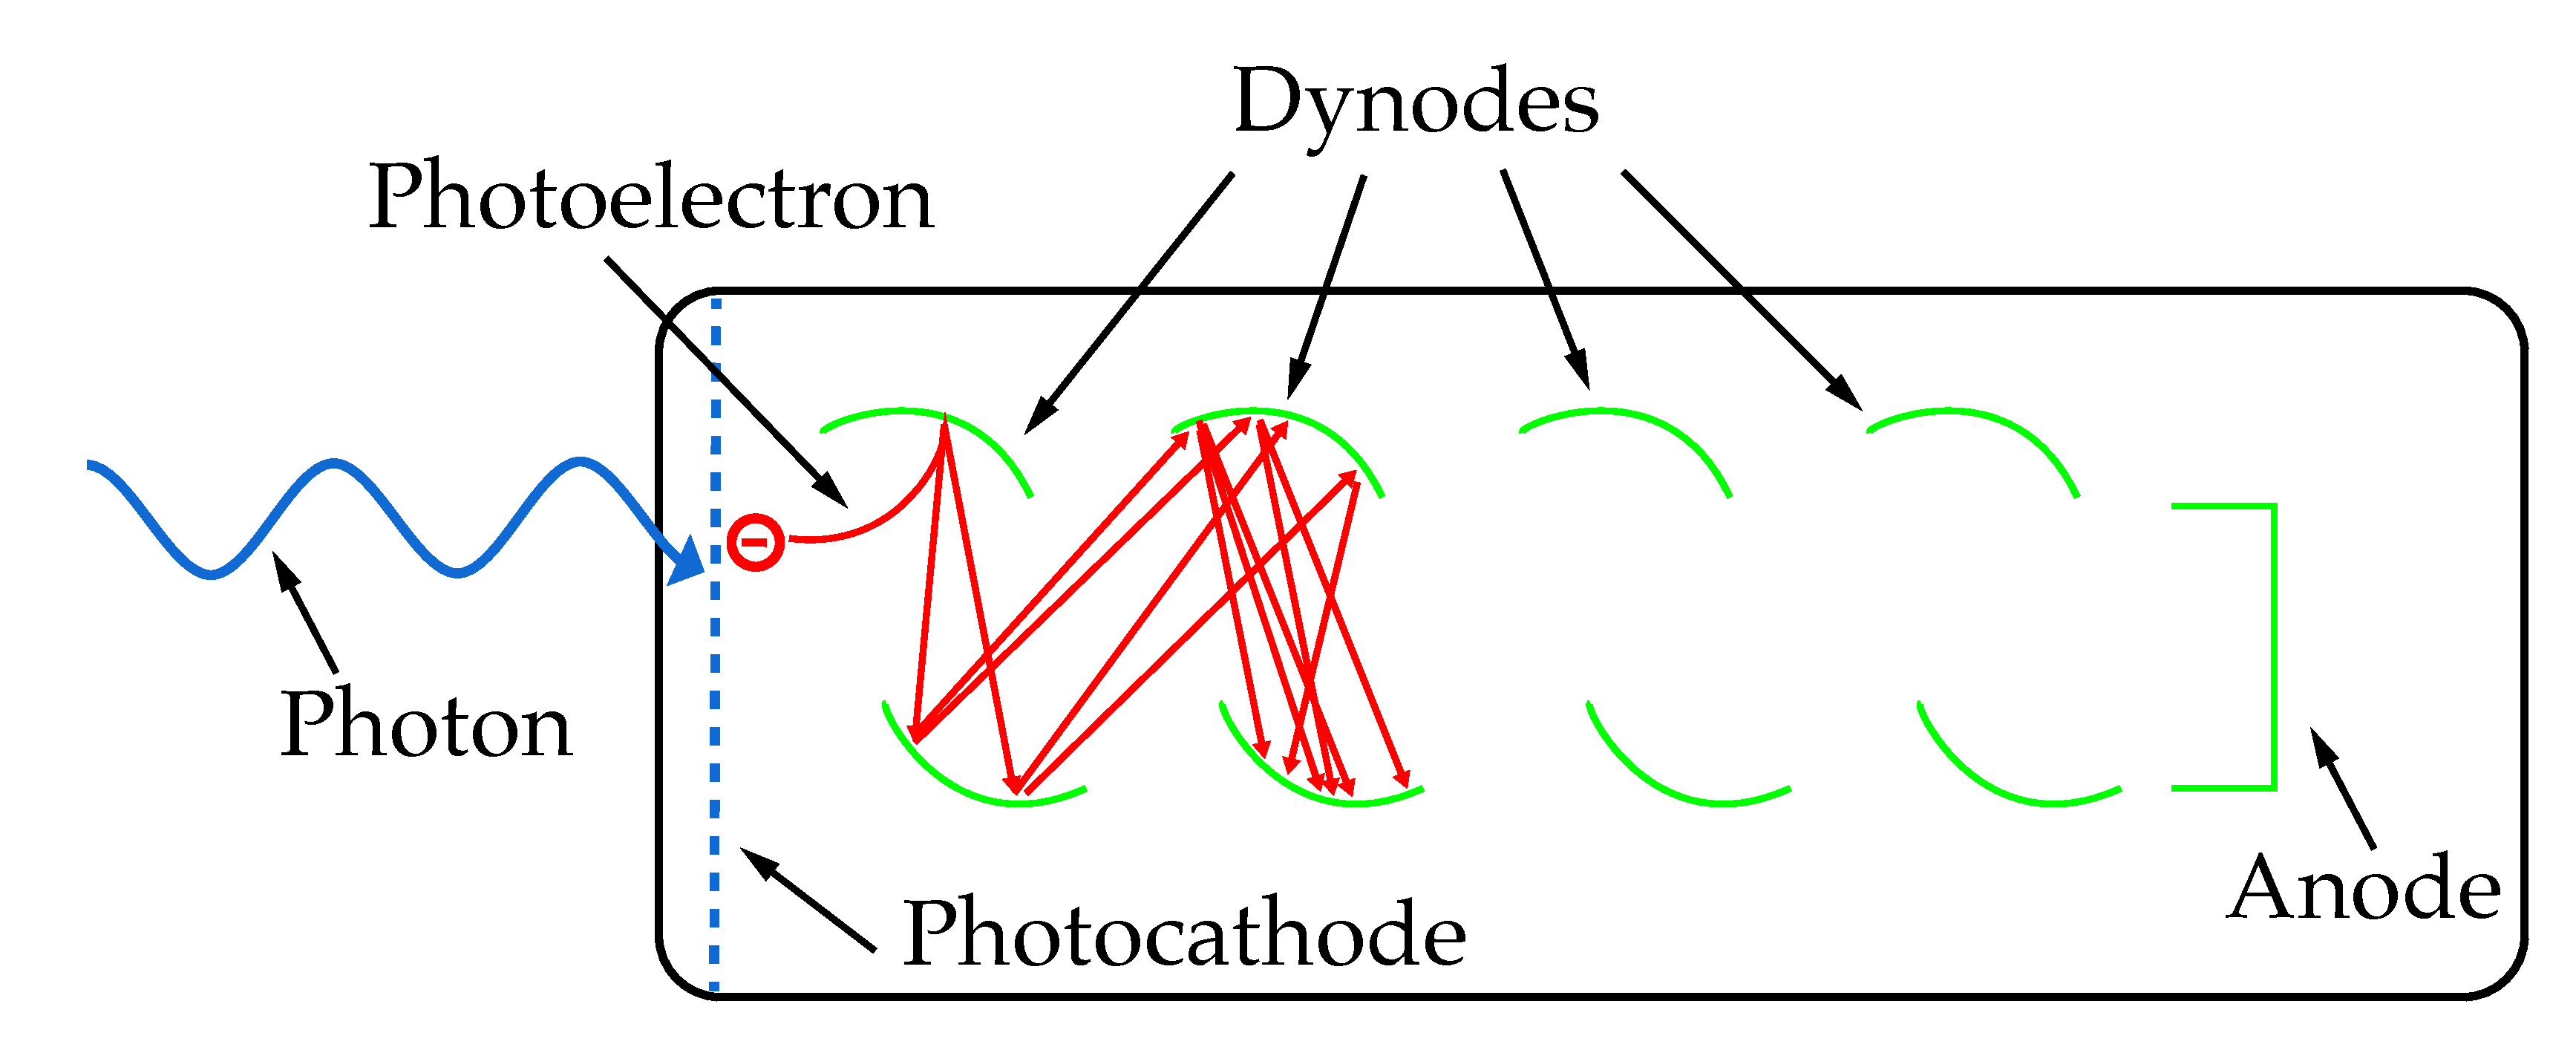
\includegraphics{ic/ic_pmt_annotated.pdf}
    \caption[PMT schematic]{A photomultiplier tube. Adapted from \cite{Bednarski2014}.}
    \labfig{pmt}
\end{figure}

As one can see in Fig. \ref{fig:pmt}, there are three principal components: a \textit{cathode}, a number of \textit{dynodes} and an \textit{anode}. When photons hit the cathode, they can release electrons via the photoelectric effect \sidecite{Einstein1905}. These photoelectrons are then accelerated (towards the right side in Fig. \ref{fig:pmt}) by an electric field within the tube. This field is generated by applying a high voltage between the cathode and the anode.

To amplify the signal, a number of \textit{dynodes} are placed between cathode and anode. These are additional electrodes with subsequently higher voltages. When the photoelectron hits the first dynode, a number of secondary electrons are generated, which are then accelerated towards the next dynode by the electric field. This process repeats for every dynode, generating an avalanche of electrons exponentially amplifying the original single photoelectron signal. The number of secondary electrons hitting the anode is proportional to the number of incident photons, resulting in a linear detector response (as long as the detector stays below its saturation limit) \sidecite{Wright2017}.

IceCube uses PMTs made by Hamamatsu Photonics (R7081-02), sensitive to photons between \SI{300}{\nm} and \SI{650}{\nm}. They have a quantum efficiency (QE) at \SI{390}{\nm} of \SI{25}{\percent}, are operated with a voltage of \SI{1500}{\V} and have a gain (electron multiplication factor) of \num{e7}. The photon-sensitive surface area is typically \SI{530}{\cm\squared} \sidecite{Abbasi2010}.

\subsection{The Digital Optical Module} \label{DOM}
\begin{marginfigure}
    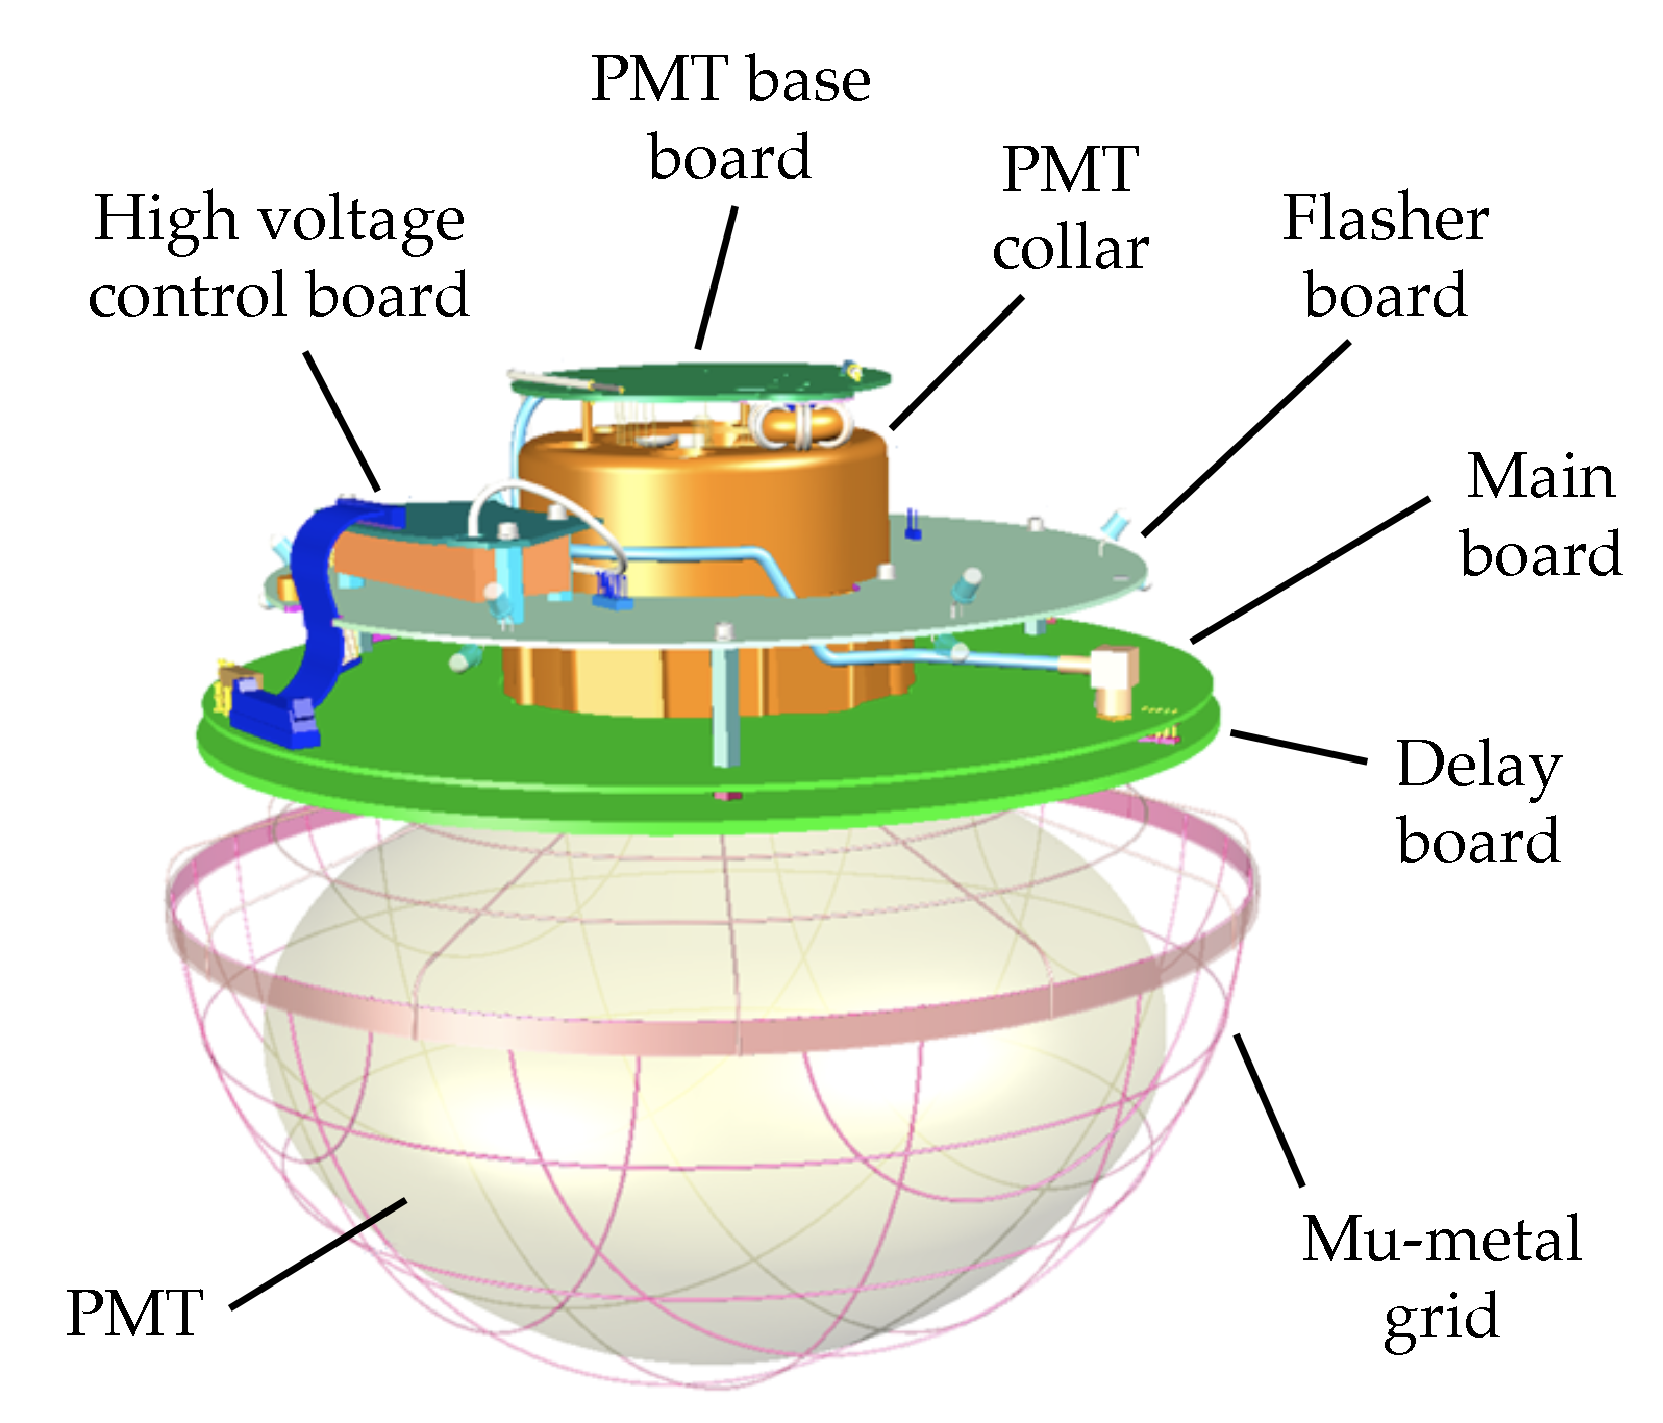
\includegraphics{ic/ic_DOM.pdf}
    \caption[IceCube digital optical module]{The IceCube DOM seen from the side. The detecting side of the PMT is facing downwards, with the main board an the PMT base board on top. From \cite{Aartsen2017}.}
    \labfig{ic_dom}
\end{marginfigure}
The individual IceCube PMTs for detecting the Cherenkov radiation are enclosed in \textit{digital optical modules} (DOMs). Each DOM consists of a pressure-resistant glass sphere, several controller boards and the PMT, facing downward (see Fig. \ref{fig:ic_dom}). The glass sphere can withstand long-term pressure of \SI{250}{\bar}. The optical transmission of the spheres was measured to be \SI{93}{\percent} at \SI{400}{\nm}, decreasing to \SI{10}{\percent} at \SI{315}{\nm}.

The circular main board hosts data acquisition and control, as well as units for communication, calibration and a power converter. Another board interfaces with the PMT, while additional boards delay the PMT signals, generate the high voltage current powering the PMT, as well as control calibration light emitting diodes (LEDs) that generate light flashes which can be received by neighboring DOMs for calibration purposes \sidecite{Aartsen2017}.
\begin{marginfigure}
    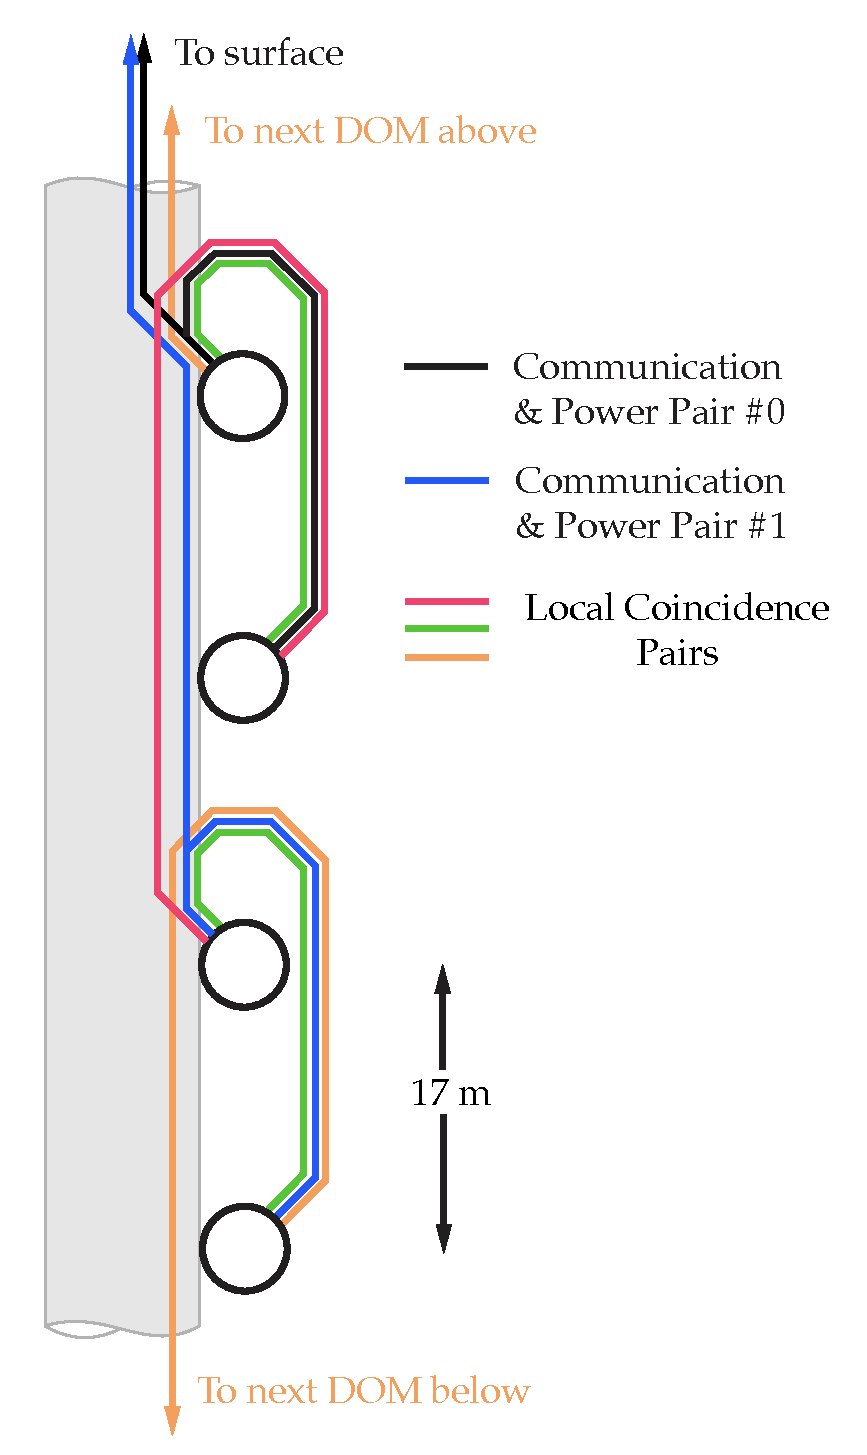
\includegraphics{ic/ic_DOM_connections.pdf}
    \caption[IceCube DOM connections]{Connection scheme for four IceCube DOMs along one string. Pairs of DOMs share one twisted-pair cable. Also, each DOM is directly connected to its direct neighbor above and below. Adapted from \cite{Aartsen2017}.} 
    \labfig{ic_dom_connections}
\end{marginfigure}
Because of data storage restrictions, the DOMs only record the full digitized waveform data after a ``hit''. A hit is triggered when also DOMs above and below the DOM in question (to be precise, the neighbors and the next-to-nearest neighbors) report a coincident signal above a certain threshold \cite{Aartsen2017}. To fully record the waveform after a hit, there needs to be some kind of buffer. This is realized with the delay board, which routes the analog PMT signal through a \SI{10}{\m} long, serpentine copper trace to delay it by \SI{75}{\nm}.

The digitization of the PMT waveform is done with the Analog Transient Waveform Digitizer (ATWD), a custom-built application specific integrated circuit (ASIC). Usually lying dormant, the ATWDs start to capture the delayed waveform when the PMT discriminator initiates it. The captured waveforms are only digitized in case a hit (i.e. local coincidence) is registered \sidecite{Abbasi2013}.

The DOMs are connected to the IceCube Laboratory (ICL) with twisted-pair copper cables. The power for the DOM is also transmitted with this cable. Two DOMs share one twisted-pair cable, and each DOM is also directly connected to its two neighbors on the same string (to detect hits, i.e. locally coincident signals). Fig. \ref{fig:ic_dom_connections} shows the connection layout.

The flasher board houses 12 LEDs operating at \SI{\sim400}{\nm} wavelength. These are used to verify the DOM timing response, to measure the DOM in-ice position, to determine the optical properties of the ice, and to verify the reconstruction algorithms \cite{Aartsen2017}.

\subsection{Detector layout}
In total, approximately 5800 DOM units were built and tested, 300 failing tests and the rest being delivered to the South Pole. The vast majority of these were ultimately deployed (5160 in total). The final detector layout (since the last drilling campaign 2010/2011, see below) consists of 86 strings. The DOMs were deployed along those strings, like pearls on a necklace. Each string contains 60 DOMs, with an average horizontal spacing between strings of \SI{125}{\meter} \cite{Aartsen2017}.

\begin{figure}
    \includegraphics[width=1.\textwidth]{ic/ic_side_view_font.pdf}
    \caption[IceCube side-on]{Side view of the IceCube detector, showing the instrumented array deep in the Antarctic glacial ice. In the center on top is the IceCube Laboratory, were data acquisition takes place. From \cite{Ahlers2018a}.}
    \labfig{ic_sideon}
\end{figure}
\begin{marginfigure}
    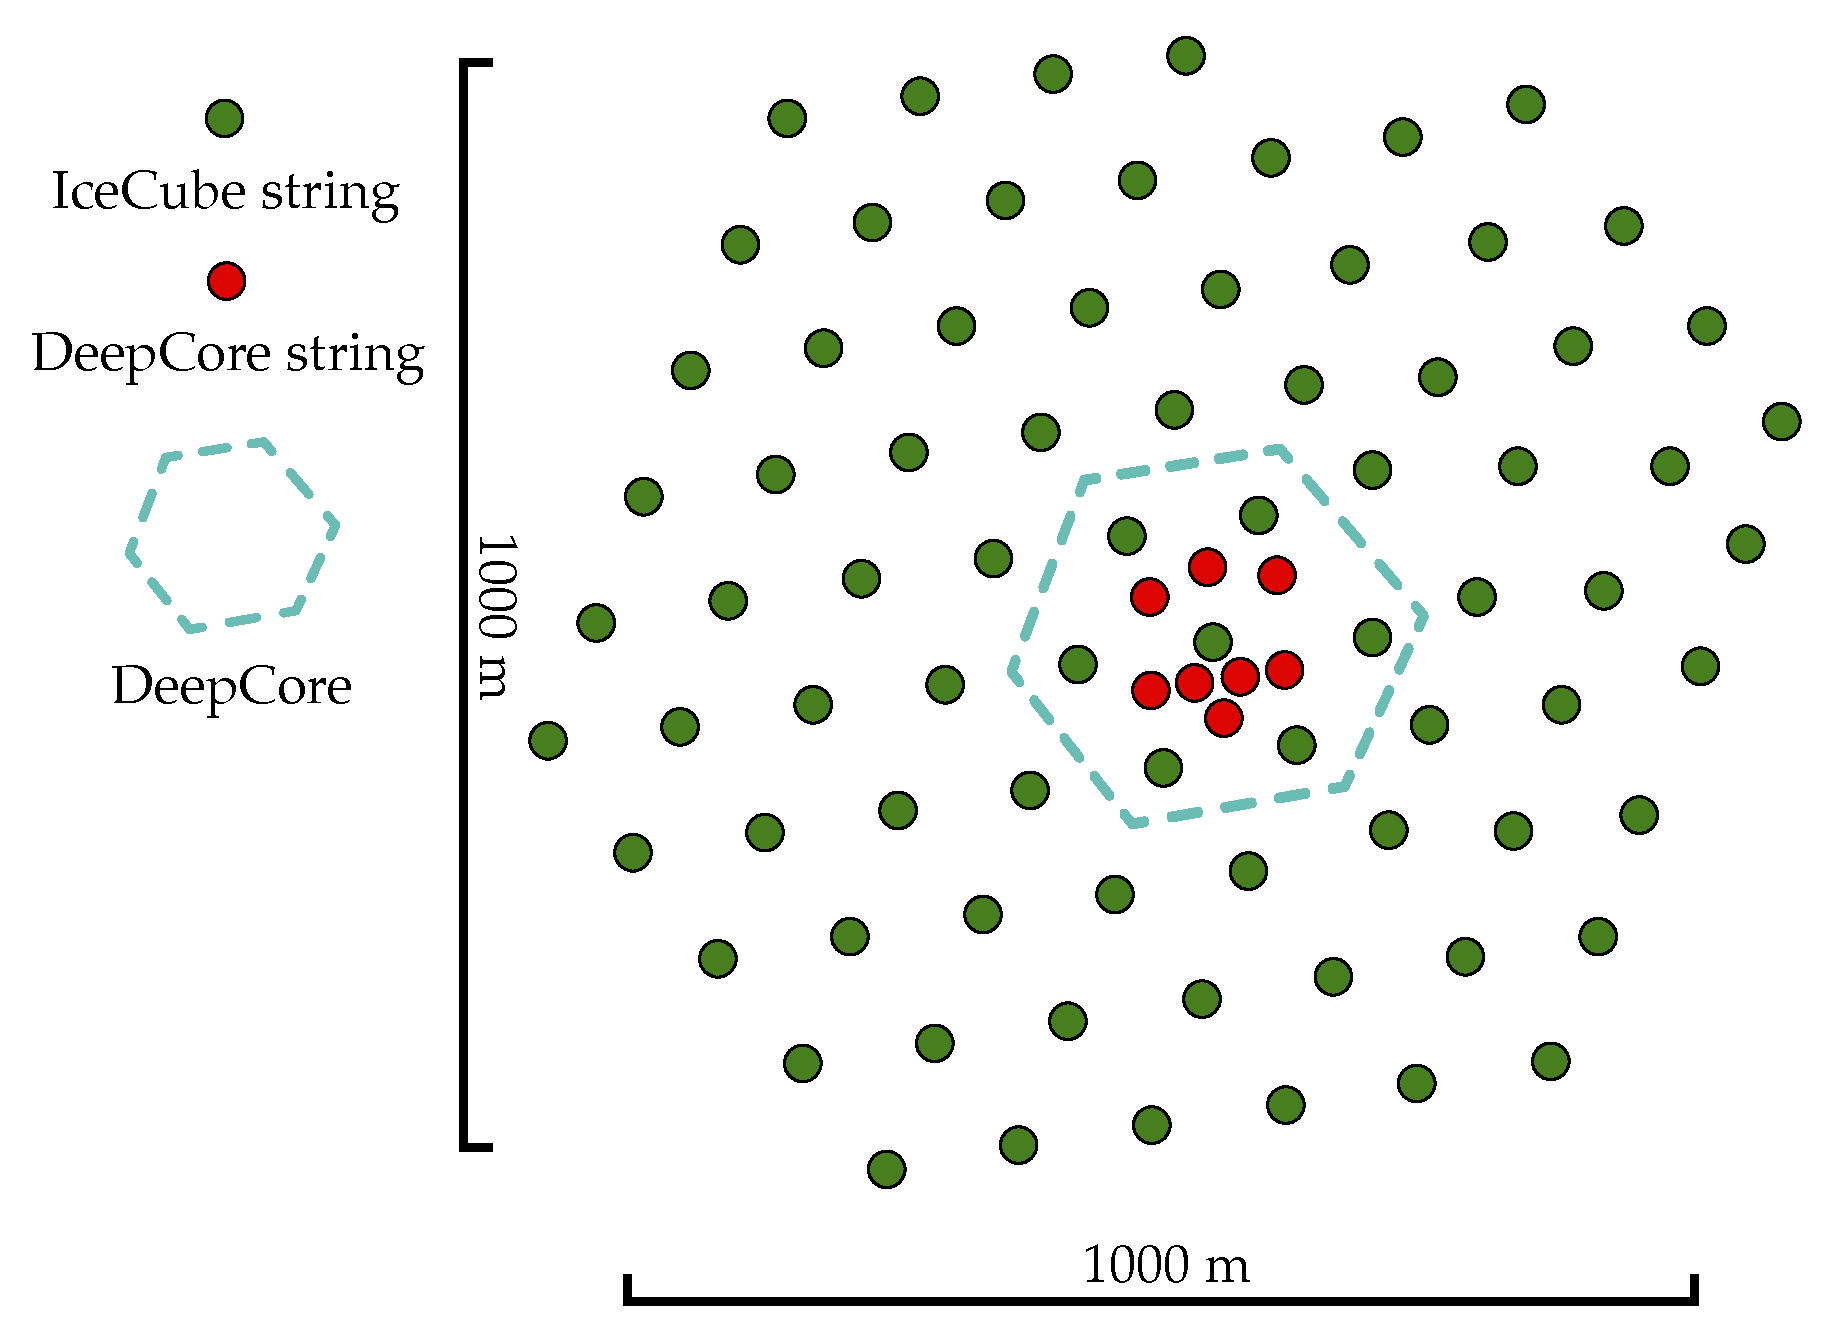
\includegraphics{ic/ic_top_view.pdf}
    \caption[IceCube top-down view]{Top-down view of the IceCube detector, spanning \SI{1}{\square\km} on the surface. From \cite{Ahlers2018a}.}
    \labfig{ic_top_down}
\end{marginfigure}

The instrumented part of the strings starts at \SI{1450}{\m} below surface, with one DOM every \SI{17}{\m} to a depth of \SI{2450}{\m}, just above the bedrock at a depth of \SI{2820}{\m}. In Fig. \ref{fig:ic_sideon} the layout of the in-ice array can be seen. The strings follow a roughly hexagonal layout (see Fig. \ref{fig:ic_top_down}), with a side length of \SI{1}{\km\squared}. The total instrumented volume of glacial ice is thus \SI{1}{\km\cubed} \cite{Aartsen2017}. Of the 5160 deployed DOMs, 92 are dead as of March 2023, a loss of \SI{1.7}{\percent}\sidenote{This is better than the predicted failure percentage, which was projected to be \SI{2}{\percent} by 2023 \cite{Aartsen2017}.}.

As can be seen in Fig. \ref{fig:ic_top_down}, there is a region in the center of the detector which is more densely instrumented: The strings are closer to each other, and also the spacing between DOMs on these strings is reduced from \SI{17}{\m} to \SIrange{7}{10}{\m}. This part of the detector is \textit{DeepCore}, designed to have a lower energy threshold of \SI{10}{\GeV}. The DOMs within DeepCore are also modified for this goal, as they are equipped with PMTs that have a \SI{35}{\percent} higher QE compared to the `normal' DOMs \cite{Aartsen2017}. 


\subsection{Deployment}
As one can imagine, embedding the DOMs within the ice was a non-trivial task. It required drilling 86 boreholes with a diameter\sidenote{The hole diameter was larger than the DOM diameter (\SI{35}{\cm}) to account for partial refreezing of the bore hole.} of roughly \SI{60}{\cm} and a length of \SI{2500}{\m}. This was achieved over several drilling campaigns with the Enhanced Hot Water Drill (EHWD) specifically built for this task. This drill had a total power of \SI{5}{\mega\W} and was able to drill with a maximum speed of \SI{2.2}{\meter\per\minute}. With these performance characteristics, one hole was drilled every \SI{48}{\hour} on average\sidenote{Drill operation happened around the clock.} \cite{Aartsen2017}. It took 7 drilling seasons to deploy the final IceCube86 setup, from the Antarctic summers 2004/2005 to 2010/2011. Fig. \ref{fig:ic_drill} shows the tower operations site directly above the bore hole \sidecite{Benson2014}.

The water for drilling the holes was heated to \SI{88}{\celsius} with 35 water heaters working in parallel, each providing \SI{125}{\kilo\W} power. The average amount of fuel used per drill hole was \SI{27000}{\liter} \cite{Benson2014}. 

\begin{figure}[]
    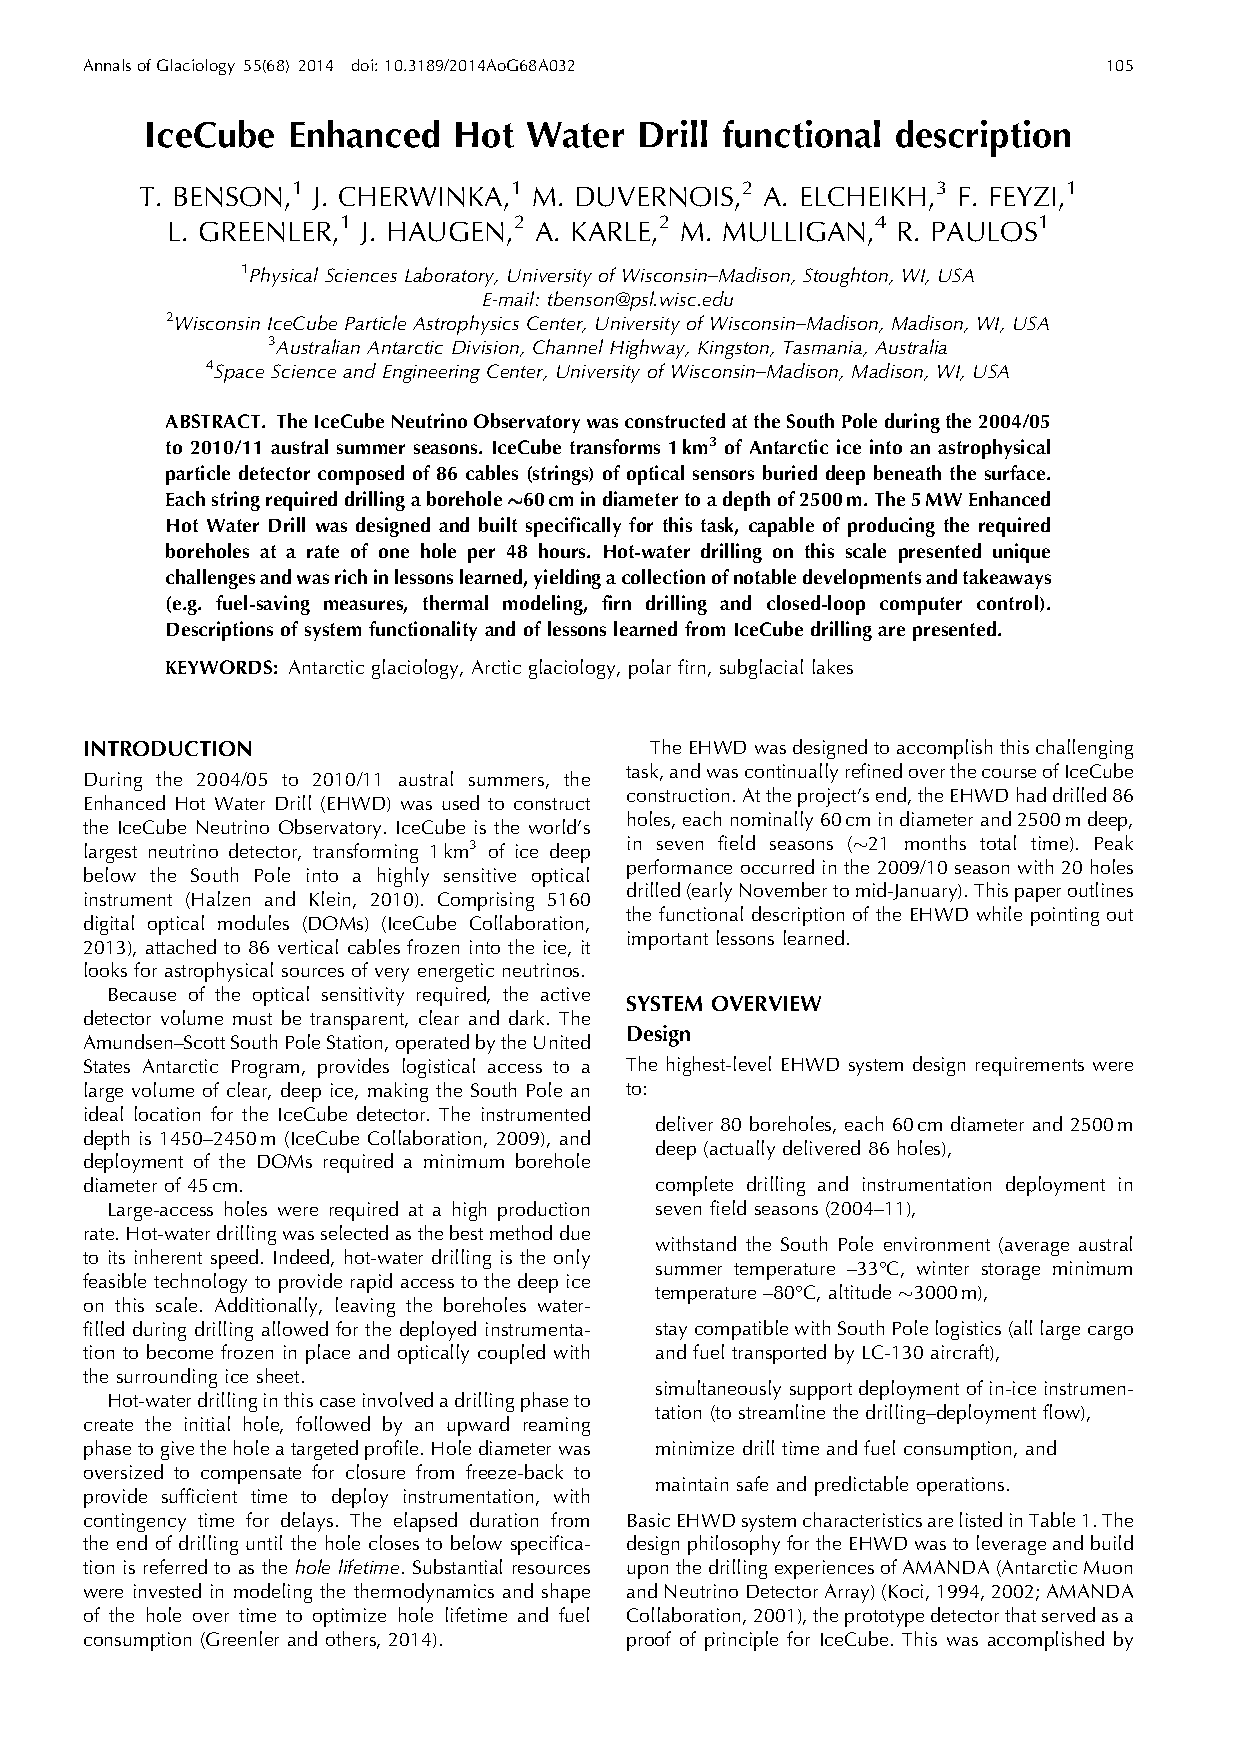
\includegraphics{ic/ic_drill.pdf}
    \caption[IceCube enhanced hot water drill]{The hole drilling part of the IceCube Enhanded Hot Water Drill, excluding the hot, pressurized water supply. One can see the tower operations site (TOS) above the hole and the hoses providing hot water and returning cooled water from the bore hole to the generators in a closed loop. From \cite{Benson2014}.}
    \labfig{ic_drill}
\end{figure}

\subsection{The IceTop surface array}
As IceCube is sensitive to particles moving fast through the ice, there is a variety of background events (see Section \ref{background}). One the major contributors are cosmic ray interactions in the atmosphere, as the muons generated in these are indiscernible from neutrino-induced muons within the in-ice array (see Section \ref{background}). IceTop serves as a partial veto against cosmic-ray muons and neutrinos, as it is sensitive to the airshowers from which they stem.

\begin{marginfigure}
    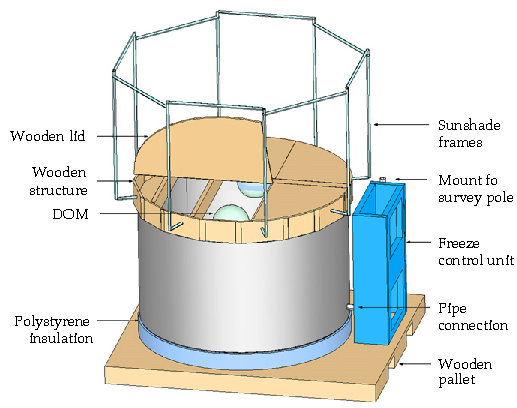
\includegraphics{ic/ic_icetop.pdf}
    \caption[IceTop detector]{IceTop surface Cherenkov detector tank. From \cite{Abbasi2013}.}
    \labfig{ic_icetop}
\end{marginfigure}

The IceTop surface array consists of $2\times81$ ice-filled Cherenkov tanks. These are placed in pairs on the same hexagonal grid as the DOM strings for the in-ice array. Each tank is equipped with two standard IceCube DOMs (see Section \ref{DOM}) \cite{Abbasi2013}, operated at two different gain levels to increase the dynamic range.\todo{more detail}

The array is sensitive to \sidecite{Aartsen2013a}.

\subsection{Data acquisition}\label{data_acquisition}
As noted above, only for locally coincident hits in multiple detectors the full waveforms are digitized by the DOMs. These are then sent to the IceCube Laboratory on the surface via the twisted-pair cable datalink, were all DOM data is ingested into the data acquisition system (DAQ). Hits throughout the detector are investigated by the system to establish common causility by temporal and sometimes spatial patterns. All hits for which common causality can be established form an \textit{event}. The rate of these events varies seasonally with the atmospheric muon flux, with a median event rate of \SI{2.7}{\kilo\Hz} and a total data rate of \SI{1}{\tera\byte\per\day} (roughly \SI{100}{\mega\bit\per\second}) \cite{Aartsen2017}.

As satellite bandwidth is limited and costly, further software triggers on-site reduce the data rate to \SI{15}{\percent} of the initial rate. These events are then transmitted via satellite to the IceCube data center at the University of Wisconsin-Madison for further analysis. The full event stream is also written to redundant disks, which are transferred twice per year to Madison.

\subsection{Time synchronization}
As precise timing information is crucial to reconstruct an event (see Section \ref{reconstruction}), all DOMs need to be synced to a common clock. This is achieved by syncing the whole system to a Symmetricom ET6000 GPS receiver. The synchronization of individual DOMs is performed once per second, while data transfer is paused during the process\sidenote{The calibration sequence takes $\lesssim$\SI{1.3}{\milli\second}} \sidecite{Abbasi2009}.

IceCube ensures temporal synchronizity with an algorithm called Reciprocal Active Pulsing (\texttt{RAPcal}): A bipolar pulse is initiated on the surface and sent to the DOM. The sender saves the local time when it sends the pulse and starts a timer. Upon reception down the string, the DOM also saves its current local time, saves the received pulse waveform, starts a timer, responds with a bipolar pulse of its own and stops the timer. Upon reception, the surface station stops its timer and requests the received pulse waveform and all timing information from the DOM.

With these six pieces of information -- the two transmit timestamps, the two receive timestamps and both waveforms -- a transformation from the GPS-synchronized surface to local DOM time domain and vice versa can be calculated, with a precision of \SIrange{1}{2}{\ns} \cite{Abbasi2009}.

\section{Angular Reconstruction}\label{reconstruction}
\begin{marginfigure}
    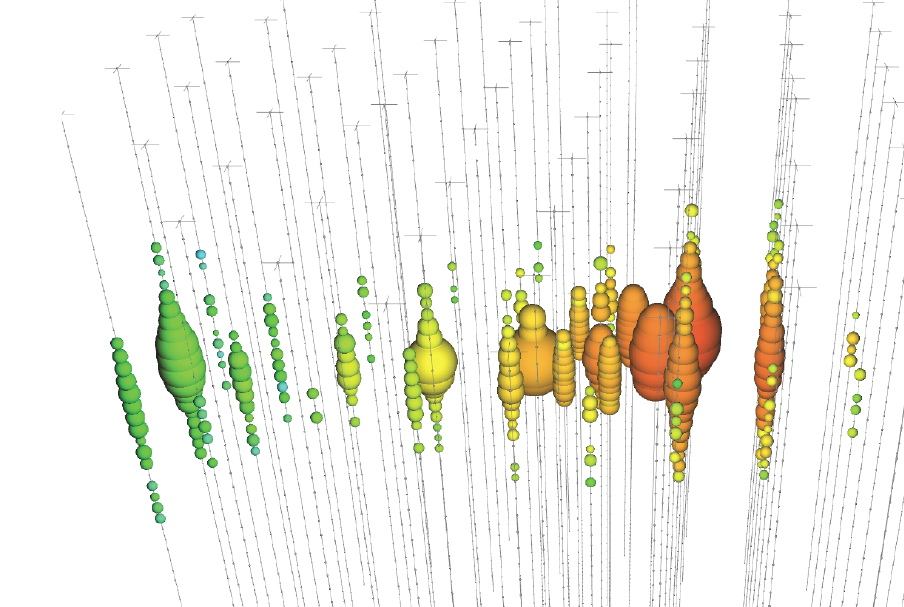
\includegraphics{ic/ic_track.png}
    \caption[Track event in IceCube]{Cascade event: The long track allows for good angular reconstruction, with high uncertainty on the event energy. From \url{masterclass.icecube.wisc.edu}.}
    \labfig{ic_track}
\end{marginfigure}
\begin{marginfigure}
    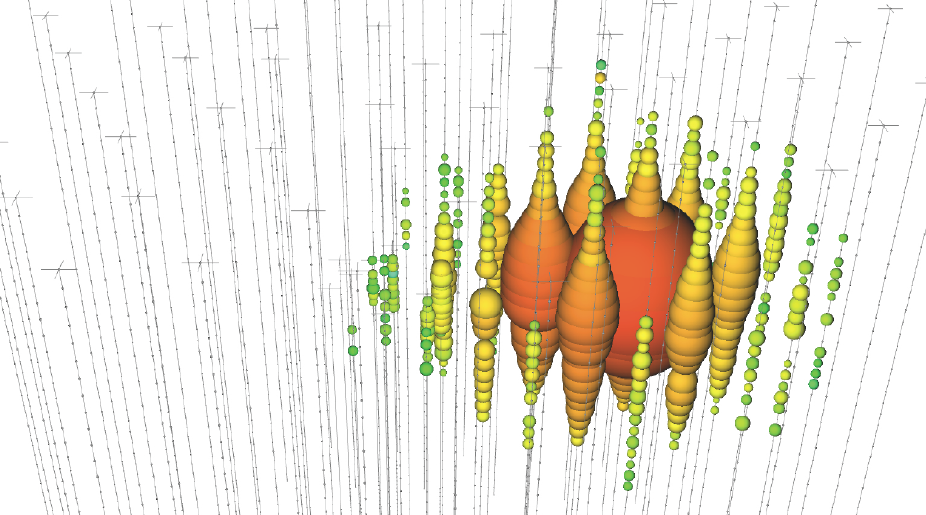
\includegraphics{ic/ic_cascade.png}
    \caption[Cascade event in IceCube]{Cascade event: The energy is fully contained in the detector, as the event is relatively isotropic. The angular uncertainty is quite large though. From \url{masterclass.icecube.wisc.edu}.}
    \labfig{ic_cascade}
\end{marginfigure}
The goal of IceCube reconstruction is twofold: Reconstructing the deposited neutrino energy, and reconstructing the neutrino arrival direction. These two goals are mutually exxclusive, which is reflected by broadly classifying the events seen by the detector in two categories: \textit{Track events} and \textit{cascade events}.

\subsection{Event types}

Track events (Fig. \ref{fig:ic_track}) are produced by secondary muons resulting from the charged-current interaction of muon neutrinos with Antarctic glacial ice\todo{ref to theory section}. They leave tracks in the ice with a length on the order of kilometers. This allows for a good angular resolution, ranging from \SI{1}{\degree} for a \SI{1}{\TeV} muon to \SI{0.3}{\degree} for a \SI{1}{\peta\eV} muon \sidecite{Abbasi2022}. The drawback is a large energy uncertainty, as parts of the muon track can lie outside the instrumented volume \sidecite{Aartsen2017a}.

Cascade events (Fig. \ref{fig:ic_cascade}) on the other hand are initiated by the charged-current interactions of $\nu_e$ and $\nu_\tau$, as well as by neutral-current interactions from neutrinos of all flavors. They are usually relatively isotropic and contained within a small fraction of the detector, as typical track lengths are of $\mathcal{O}(\SI{10}{\meter})$. Their relative isotropicity only allows for poor angular resolution (\SIrange{10}{15}{\degree}), but comparably good energy reconstruction ($\frac{\delta E}{E} \approx \SI{15}{\percent}$) \cite{Aartsen2017a}.

As this thesis is mainly interested in the sources of high-energy astrophysical neutrinos, the track events are more important here, and I will focus on the angular reconstruction of those.

\subsection{Likelihood approach}
The basic angular reconstruction algorithm for muon tracks used in IceCube is based on the work done for AMANDA. It is based on a maximum-likelihood method \sidecite{Ahrens2004}. This can be understood as follows: Given a set set of unknown track parameters $\vec{a}$ and a set of experimentally determined values $\vec{x}$, what values of the unknown parameters do maximize the probability of measuring the actually observed values of $\vec{x}$?

This likelihood is denoted $\mathcal{L}(\vec{x}|\vec{a})$. If the components $x_i$ of $\vec{x}$ are independent, it can be expressed as

\begin{equation}
\mathcal{L}(\vec{x}|\vec{a}) = \prod_i p(x_i|\vec{a})
\end{equation}

Here, $p(x_i|\vec{a})$ is the probability density function (PDF) of measuring $x_i$ given a set of parameters $\vec{a}$. Maximizing $\mathcal{L}$ when varying $\vec{a}$ (or, for technical reasons, minimizing $-\log{\mathcal{L}}$) results in the most likely set of unknown parameters $\vec{a}$, and we are done with the reconstruction.

\subsection{Parametrization}
\begin{figure}[h!]
    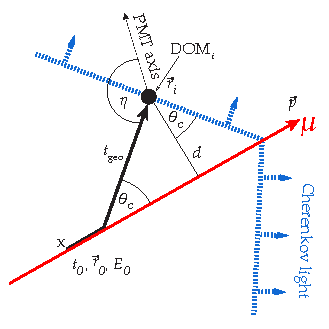
\includegraphics[width=0.7\textwidth]{ic/amanda_reco.pdf}
    \caption[Angular reconstruction in IceCube]{Parametrization for the angular muon reconstruction. Adapted from \cite{Ahrens2004}.}
    \labfig{ic_reco_cherenkov}
\end{figure}

To simplify matters, we assume that we are dealing with a muon with maximum allowed speed ($\beta=1$), travelling along a track of infinite length. Furthermore, we neglect stochastic photon losses. The set of parameters $\vec{a}$ needed to describe the physical situation in the detector are visualized in Fig. \ref{fig:ic_reco_cherenkov}: $\vec{a}$ = ($t_0$, $E_0$, $\vec{r_0}$, $\vec{p}$). They describe the trajectory of a muon at time $t_0$ with energy $E_0$ at position $\vec{r_0}$, traveling in the direction $\vec{p}$. So we are dealing with one time parameter, one energy parameter and positional parameters in 5 dimensions, where the vertex position $\vec{r}_0$ can be expressed in (x,y,z) and the muon direction $\vec{p}$ is usually described by two angles, zenith and azimuth\sidenote{The zenith angle is the angle to a line vertical to the earth, centered on the detector surface and pointing southwards. An azimuth angle of \SI{90}{\degree} describes a particle traveling from North (prime meridian pointing towards Greenwich) to South, while an azimuth angle of \SI{0}{\degree} travels from the 90th Meridian East to West.}. In the context of IceCube muon reconstruction, this parameter set $\vec{a}$ is known as the \textit{track hypothesis}.

Now, a DOM in the detector at position $\vec{r}_i$ with a distance $d$ to the track can be hit by Cherenkov photons emitted by the muon traveling along the track with the Cherenkov angle $\theta_\text{C}$, arriving at an angle $\eta$ with respect to the PMT axis. Without scattering, the photon reaches the $\text{DOM}_i$ at the geometrical time $t_\text{geo}$, which can be expressed as follows:
\begin{equation}
t_\text{geo} = t_0 + \frac{|\vec{p}\cdot(\vec{r_i}-\vec{r_0})|+d\cdot \tan{\theta_\text{C}}}{c_0}
\end{equation}
with $c_0$ the vacuum speed of light. As this does not take scattering into account, it is useful to define a relative time of arrival, the \textit{time residual} $t_\text{res} = t_\text{hit} - t_\text{geo}$. This is the additional time introduced by scattering as opposed to a Cherenkov photon travelling directly from the muon to the DOM.

As the position of the DOM is known, $t_\text{res}$ is the most significant observable for each DOM,  We therefore simplify $x_i$ to $t_{\text{res},i}$, and express $\vec{a}$ as a function of the individual DOM parameters: $\vec{a}= (d_i,\eta_i,...)$.



\subsection{First (single) photoelectron fit}
Matters can be simplified further. While the muon is travelling and emitting Cherenkov light, multiple photons can hit each DOM. One simplification is to only regard the \textit{first} photon hitting an individual DOM, as it is usually less scattered than the average photon. If the reconstruction is carried out with this simplification, it is called \textit{single photoelectron} (SPE) fit. The likelihood function for this is:\sidenote{As stated above, this already includes the reduction of $x_i$ to $t_{\text{res},i}$.}

\begin{equation}
\mathcal{L}_\text{1st}(\vec{x}|\vec{a}) = \prod_i^\text{1st hits} p(t_{\text{res},i}|\vec{a}=d_i, \eta_i,...)
\end{equation}
where the probability density function $p(t_{\text{res},i}|\vec{a})$ is obtained from simulations modeling the photon propagation through the Antarctic ice (this is necessary because the photon scatter needs to be accounted for). The simulation results are either stored in look-up tables or approximated by analytical functions \cite{Ahrens2004}. 

\subsection{Multi photoelectron fit}
A complication is that one expects the first photon in a DOM detecting multiple photons \textit{earlier} than a photon detected by a DOM only registering a single photon (more hits equal proximity to the event, and therefore a higher signal. The event is detected better and therefore earlier). 

This leads to the \textit{multi photoelectron} (MPE) fit. Here, the single photon part of the likelihood is modified by the cumulative PDF (CDF), which is given by\todo{explain!!}
\begin{equation}
P(t_{\text{res},i}|\vec{a}) = \int^{\infty}_{t_{\text{res},i}}p(t|\vec{a})\,dt
\end{equation}
Using this, the MPE likelihood is given as
\begin{equation}
\mathcal{L}_\text{MPE} = \prod_i^\text{1st hits} p(t_{\text{res},i}|\vec{a}) \cdot N_i \cdot (1-P(t_{\text{res},i}|\vec{a})^{N_i-1}
\end{equation}
where $N_i$ is the total number of photons recorded by $\text{DOM}_i$ \cite{Ahrens2004}.\todo{Überleitung!}

\subsection{Millipede reconstruction} \label{millipede}
High-energy neutrion alerts that make the realtime alert cuts (see Section \ref{ic_alert_program}) are subjected to a computationally intensive algorithm dubbed \texttt{Millipede}, as it promises higher reconstruction fidelity. Due to its demand of computational resources it is only run for selected events at the IceCube data center in Madison.

\begin{marginfigure}
    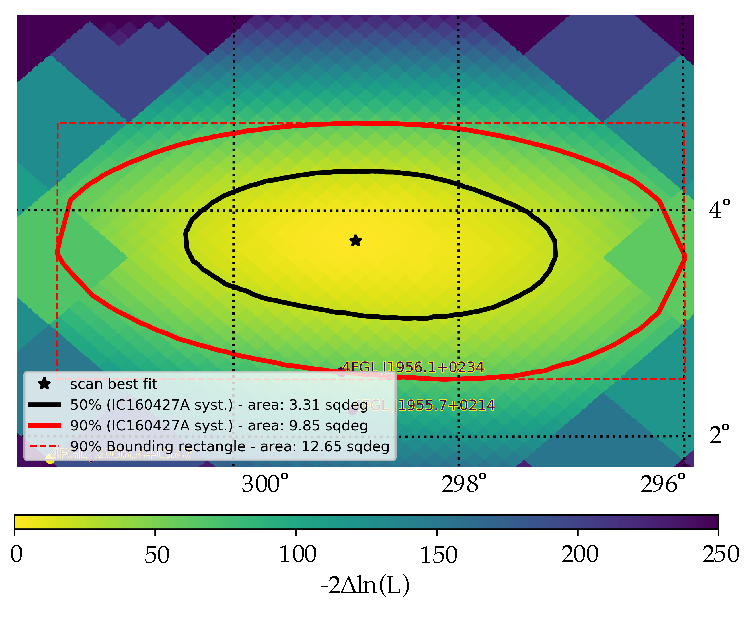
\includegraphics[width=1\textwidth]{ic/ic_millipede_IC221124A.pdf}
    \caption[\texttt{Millipede} reconstruction of IC221124A]{\texttt{Millipede} reconstruction of IC221124A.}
    \labfig{ic_millipede}
\end{marginfigure}

This reconstruction consists of a maximum likelihood scan covering the whole sky. To allow scanning, the sky is pixelated into grids of increasing resolution following the Hierarchical Equal Area isoLatitude Pixelation (\texttt{HEALPix}) scheme \sidecite{Gorski2005}. Each pixel of specific resolution covers the same area on the sky. For each scanned pixel, the muon direction is fixed to originate from that sky location.

For this fixed direction, the likelihood of the deposited energy resulting from the best fit and the neutrino interaction vertex in the detector are then computed. Pixels near the likelihood maximum are then subdivided with a finer \texttt{HEALPix} resolution. This procedure ultimately results in a likelihood map of the sky, with increasing granularity towards the global maximum \sidecite{Abbasi2023}.

To compute \SI{50}{\percent} and \SI{90}{\percent} confidence level uncertainty contours, Monte Carlo re-simulations from IC160427A are used. For this event, Pan-STARRS found a possible counterpart, PS16cgx\sidenote{Spectroscopic follow up reveiled that this can either be a SN Ic, which would be compatible with neutrino production, or -- more likely -- a SN Ia, which would exclude it as a neutrino source.} \sidecite{Kankare2019}.

In the re-simulations, the systematic parameters of the antarctic ice used to model photon propagation were varied. Each re-simulated event was fit with \texttt{Millipede}. The distribution of differences between the best-fit likelihood and the ground truth of the simulated event can then be employed to convert the change in log-likelihood over the map to a confidence level.

Currently, all pixels that satisfy $\log \mathcal{L}_\text{min}-\log \mathcal{L}_\text{pixel} = -11.3$ $(-32.1)$ form the \SI{50}{\percent} (\SI{90}{\percent}) error contours \sidecite{Gualda2021}. In Fig. \ref{fig:ic_millipede} these contours are displayed for an example event. The black line shows the \SI{50}{\percent} uncertainty region, while the red line shows the \SI{90}{\percent} area. \todo{Cristina input}

\section{The Realtime Alert Program}\label{ic_alert_program}
Since 2016, IceCube is hosting a realtime alert program, providing the astrophysical community with low-latency, high-quality astrophysical neutrino alerts \cite{Aartsen2017a}. This program saw a major revision in 2019, when two new alert streams, namely \textit{Gold} and \textit{Bronze}, were created \sidecite{Tung2019}. As all alerts used within this work except one stem from this revised system, I will focus on presenting the newer alert scheme.

\subsection{Background}\label{background}
Depending on the declination, there are two major sources of background events in the IceCube detector, both stemming from secondary cosmic ray particles from the earth's atmosphere.
\begin{figure}[htb]
    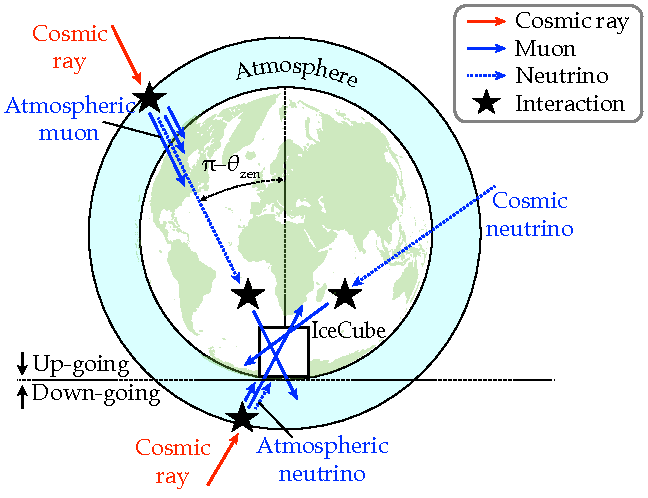
\includegraphics[width=0.8\textwidth]{ic/ic_background.pdf}
    \caption[Background events]{Background events in the detector. Cosmic rays hit the atmosphere around the globe and produce muons (solid blue arrows), as well as neutrinos (dashed blue arrows). When constraining to \textit{up-going} events from the norther hemisphere, the detector is shielded form atmospheric muons, but not atmospheric neutrinos, as these can traverse the earth. Adapted from \cite{Ahlers2018a}.}
    \labfig{ic_background}
\end{figure}

\begin{marginfigure}
    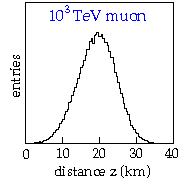
\includegraphics[width=0.8\textwidth]{ic/ic_muon_free_path.pdf}
    \caption[Muon free path in ice]{Free path length for \SI{1}{\peta\eV} muons in ice. The mean free path in ice is slightly longer than in rock. From \cite{Chirkin2004}.}
    \labfig{ic_muon_free_path}
\end{marginfigure}

\textbf{Atmospheric muons} are created by cosmic rays hitting the atmosphere. One can efficiently filter this background by restricting the analysis to \textit{up-going} muon tracks. These are tracks that come from the bottom of the detector, i.e. the northern hemisphere. Atmospheric muons stemming from cosmic ray events in the northern hemisphere are filtered out by the earth's core (see Fig. \ref{fig:ic_background}), as the mean free path of muons within the earth is much smaller \sidecite{Chirkin2004} than the distance they have to cross (see Fig. \ref{fig:ic_muon_free_path}). Note that due to light scattering within the ice, some down-going tracks can be misclassified as up-going \sidecite{Ahlers2018a}.

One complication here stems from the fact that the earth starts to become opaque for neutrinos of higher energies. Studies interested in \si{\peta\eV} neutrinos therefore must deal with the fact that these get the more suppressed the longer their path through the earth is. E.g. a \SI{1}{\peta\eV} neutrino with a zenith angle of \SI{140}{\degree} is absorbed with \SI{90}{\percent} probability \sidecite{Aartsen2017c}.

\begin{marginfigure}
    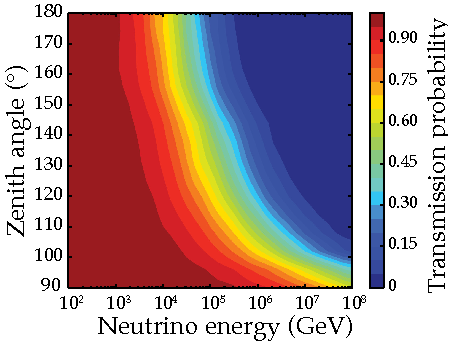
\includegraphics{ic/ic_absorption_earth.pdf}
    \caption[Neutrino absorption in the earth]{Neutrino transmission probability through the earth. The longer the distance travelled (higher zenith angles) and the higher the neutrino energy, the more likely is absorption. From \cite{Aartsen2017c}.}
    \labfig{ic_absorption_earth}
\end{marginfigure}

\textbf{Atmospheric neutrinos} also stem from cosmic ray showers. These are cannot be suppressed by directional cuts, creating an irreducible background: When atmospheric neutrinos cross the earth and interact with the matter close to the detector, they can produce muons indistinguishable from muons created by `proper' cosmic neutrinos \cite{Ahlers2018a}.

\subsection{Event selection} \label{ic_event_selection}
Gold and bronze alerts are drawn from three different selection schemes, originally designed to cater to different science goals. These are \textbf{High Energy Starting Events} (HESE), \textbf{Extremely High Energy} (EHE) events and \textbf{Gamma-Ray Follow Up} (GFU) events.

\textbf{HESE} are events that start \textit{within} the detector. This is guaranteed by using the outer regions of the detector as a veto region, in which (almost) no Cherenkov light must be detected \sidecite{Aartsen2013}. The sizes of those regions can be seen in Fig. \ref{fig:ic_hese_veto}. The majority of HESE events are cascades and therefore not well suited for observational follow-up. Because of this, additional cuts are applied: The reconstruction must favor a track interpretation of the event, and the reconstructed track length must exceed \SI{200}{\meter} \cite{Tung2019}.
\begin{marginfigure}
    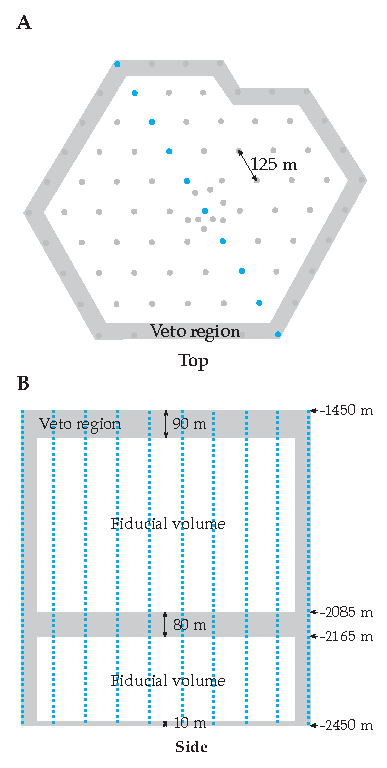
\includegraphics{ic/ic_HESE_veto.pdf}
    \caption[HESE veto regions]{High-energy starting events veto regions. The strings marked in blue in the top-down view at the top (A) show the location of the side view, displayed at the bottom (B). From \cite{Aartsen2013}.}
    \labfig{ic_hese_veto}
\end{marginfigure}

\textbf{EHE} events must contain at least 4000 photoelectrons, aiming at neutrino energies of \SIrange{0.5}{10}{\peta\eV}. Additionally, a $\chi^2$-based goodness-of-fit cut is applied to select track-like events with good reconstructions. Lastly, a cut depending on the zenith angle is also applied on the number of photoelectrons required \cite{Tung2019}.

\textbf{GFU} events are selected based on a boosted decision tree trained to identify \textit{through-going} (as opposed to `starting') track events with astrophysical origin. Energy cuts are applied: Northern hemisphere events are selected based on their reconstructed muon energies, while from the southern hemisphere are selected based on the total photoelectron charge deposited in the detector.

The cuts from all three event pools are gauged to achieve two different values of \textit{signalness}, which is a proxy for the probability that the event is of astrophysical origin \cite{Tung2019}. It is defined as follows:
\begin{definition}\label{signalness_def}
$\text{Signalness}(E,\theta_\text{zen}) = \frac{N_\text{signal}(E,\theta_\text{zen})}{N_\text{signal}(E,\theta_\text{zen})+N_\text{background}(E,\theta_\text{zen})}$
\end{definition}
where $\theta_\text{zen}$ is the zenith angle and $E$ is the respective energy proxy of the event selections described above.

The cuts on the individual event selections are tuned to ensure that \textit{gold} alerts on average have a signalness $>\SI{50}{\percent}$, and \textit{bronze} alerts have a signalness $>\SI{30}{\percent}$.
\subsection{Alert distribution} \label{ic_alerts}
All events that pass a first stage of filtering are sent to the IceCube data center (see Section \ref{data_acquisition}) via Iridium satellite to minimize latency. There, their signalness is computed. If they make either the gold or the bronze selection, they are distributed globally with the Gamma-Ray Coordinates Network (GCN) in the form of GCN Notices.
\begin{marginfigure}
    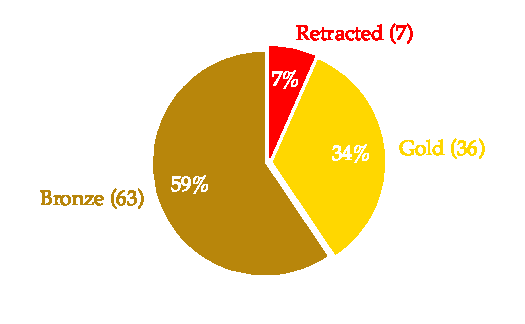
\includegraphics{ic/ic_he_alert_overview.pdf}
    \caption[IceCube alert overview]{High-energy neutrino alerts issued by IceCube since start of the new alert stream in June 2019.}
    \labfig{ic_he_alert_overview}
\end{marginfigure}
Each notices contains the discovery time, a unique event number, the reconstructed direction in right ascension (RA) and declination (Dec) of the candidate neutrino, a statistical error for the direction, the reconstructed neutrino energy, the signalness and the false alarm rate \cite{Tung2019}.

Those information are later appended by \texttt{Millipede}, a computationally more demanding, but more sophisticated reconstruction, which is initiated manually (see Section \ref{millipede}. These are typically distributed a few hours after the initial notice in the form of a GCN circular \cite{Tung2019}.

As of March 2023, a total of 106 events have been distributed in this format, with 7 later being retracted. Since the start of the gold and bronze alert stream in June 2019, this amounts to $2.2$ non-retracted alerts per month\sidenote{This is quite close to the 2.5 alerts per month predicted in \cite{Tung2019}.} (0.8 gold alerts, 1.4 bronze alerts).

If the event is most likely astrophyiscal and reasonably well pin-pointed, one can scan the sky localization with a telescope and look for potential sources of the neutrino. But where to obtain optical information from? The instrument used for this, the Zwicky Transient Facility, will be described in the next chapter.